\documentclass{article}
\usepackage{amsmath}
\usepackage{amssymb}
\usepackage{indentfirst}
\usepackage{graphicx}
\usepackage{color}
\usepackage{fancyhdr}
\usepackage{epstopdf}
\usepackage{indentfirst}
\usepackage{geometry}
\usepackage{bm}
\geometry{left=2.5cm,right=2.5cm,top=2.5cm,bottom=2.5cm}

\title{8.511 Problem Set 6}
\author{Yijun Jiang}
%\email{yjjiang@mit.edu}
\date{\today}

\pagestyle{fancy}
\lhead{Yijun Jiang}
\rhead{8.511 Problem Set 6}

\begin{document}
\maketitle
\section{Breakdown of Semiclassical Theory: Zener Tunneling}
\subsection{Part (a)}
Since the potential $V(x)$ is perodic, we can expand it into discrete Fourier components,
\begin{equation*}
V(x)=\sum_GV_Ge^{iGx}
\end{equation*}

The Fourier transform of $\Psi(x)$ is (suppose the system is finite, so the integral is replaced by a summation)
\begin{equation*}
\Psi(x)=\sum_ka_ke^{ikx}
\end{equation*}
where in general $k$ is complex. Plugging these expansions into the Schr\"{o}dinger equation, we have
\begin{equation*}
\sum_k\frac{\hbar^2k^2}{2m}a_ke^{ikx}+\sum_k\sum_GV_Ga_{k-G}e^{ikx}=\sum_kEa_ke^{ikx}
\end{equation*}

We can see that only those $k$ differ by $G$ are coupled.
\begin{equation*}
\frac{\hbar^2k^2}{2m}a_k+\sum_GV_Ga_{k-G}=E_ka_k
\end{equation*}

The corresponding wavefunction can be labelled as $\Psi_k$, where $\textup{Re}(k)$ is taken within the first Brillouin zone.
\begin{equation*}
\Psi_k(x)=\sum_Ga_{k-G}e^{i(k-G)x}
\end{equation*}

In the vicinity of the zone boundary, the Fourier component $k=G_0/2+\kappa$ is near degenerate with $k'=-G_0/2+\kappa$. The coupling between these two states is $V_{G_0}$. Therefore, the truncated Hamiltonian is
\begin{align*}
H&=\left(\begin{array}{cc}\frac{\hbar^2}{2m}\left(\frac{1}{2}G_0+\kappa\right)^2&V_{G_0}\\V_{G_0}^*&\frac{\hbar^2}{2m}\left(-\frac{1}{2}G_0+\kappa\right)^2\end{array}\right)\\
&\approx E_0I+\left(\begin{array}{cc}\frac{\hbar^2}{2m}G_0\kappa&V_{G_0}\\V_{G_0}^*&-\frac{\hbar^2}{2m}G_0\kappa\end{array}\right)\\
\end{align*}

$E_0+\varepsilon$ is an eigenvalue. Therefore,
\begin{equation*}
\left|\begin{array}{cc}\frac{\hbar^2}{2m}G_0\kappa-\varepsilon&V_{G_0}\\V_{G_0}^*&-\frac{\hbar^2}{2m}G_0\kappa-\varepsilon\end{array}\right|=0
\end{equation*}
which simplifies to
\begin{align*}
\kappa^2&=\frac{\varepsilon^2-|V_{G_0}|^2}{\left(\frac{\hbar^2G_0}{2m}\right)^2}\\
&=\frac{2m}{\hbar^2}\left(\frac{\varepsilon^2-|V_{G_0}|^2}{4E_0}\right)\\
\end{align*}

\subsection{Part (b)}
%When the electron tunnels, its $\kappa$ changes with $x$, such that its total energy is conserved. From A in the valance band to B in the conduction band, the energy gap $\Delta$ must be compensated by the electric potential $eEd_{AB}$. Therefore, the distance between $A$ and $B$ is thus $d_{AB}=\Delta/eE$.
%
Inside the band, $\kappa(x)$ is real. During the tunneling, $\kappa(x)$ is imaginary. At the start and the end of tunneling, $\kappa$ must reach its critical value, which is 0. This gives $(eEx_A)^2=(eEx_B)^2=|V_{G_0}|^2$. Therefore,
\begin{align*}
&x_A=-\frac{|V_{G_0}|}{eE}=-\frac{\Delta}{2eE}\\
&x_B=\frac{|V_{G_0}|}{eE}=\frac{\Delta}{2eE}\\
&d=x_B-x_A=\frac{2|V_{G_0}|}{eE}=\frac{\Delta}{eE}
\end{align*}

\subsection{Part (c)}
%\begin{equation*}
%\varepsilon_{\pm}(x)=\sqrt{\frac{\hbar^2}{2m}4E_0\kappa^2(x)+\left(\frac{\Delta}{2}\right)^2}
%\end{equation*}
%
%During the tunneling, the change in the energy gap must be compenstated by the electric potential.
%\begin{equation*}
%\varepsilon_+-\varepsilon_-=\Delta-eE(x_B-x)
%\end{equation*}
%
%Therefore,
%\begin{align*}
%\kappa(x)&=\sqrt{\frac{m}{8E_0\hbar^2}\left((\Delta-eE(x_B-x))^2-\Delta^2\right)}\\
%&=\frac{i\Delta}{2\hbar}\sqrt{\frac{m}{2E_0}\left(1-\left(1-(x_B-x)/d_{AB})^2\right)\right)}
%\end{align*}
%
%Let $x'=x_B-x$.
%\begin{equation*}
%|\kappa(x)|=\frac{\Delta}{2\hbar}\sqrt{\frac{m}{2E_0}\left(1-\left(1-(x'/d_{AB})^2\right)\right)}
%\end{equation*}
%
%Therefore,
%\begin{align*}
%P&=\exp\left(-2\int_A^B|\kappa(x)|dx\right)\\
%&=\exp\left(-\frac{\Delta}{\hbar}\sqrt{\frac{m}{2E_0}}\int_0^{d_{AB}}\sqrt{\left(1-\left(1-(x'/d_{AB})^2\right)\right)}dx'\right)\\
%&=\exp\left(-\frac{\Delta^2}{\hbar eE}\sqrt{\frac{m}{2E_0}}\int_0^1\sqrt{1-(1-x'')^2}dx''\right)\\
%&=\exp\left(-\frac{\Delta^2}{\hbar eE}\sqrt{\frac{m}{2E_0}}\frac{\pi}{4}\right)
%\end{align*}
%
Let $\varepsilon(x)=eEx$. Then during the tunneling,
\begin{equation*}
|\kappa(x)|=\sqrt{\frac{2m}{4E_0\hbar^2}\left(|V_{G_0}|^2-(eE)^2x^2\right)}
\end{equation*}

Therefore,
\begin{align*}
\int_{x_A}^{x_B}|\kappa(x)|dx&=\sqrt{\frac{2m}{4E_0\hbar^2}}\int_{-|V_{G_0}|/eE}^{|V_{G_0}|/eE}\sqrt{|V_{G_0}|^2-(eE)^2x^2}dx\\
&=\sqrt{\frac{m}{2E_0\hbar^2}}\frac{|V_{G_0}|^2}{eE}\int_{-1}^1\sqrt{1-x'^2}dx'\\
&=\sqrt{\frac{m}{2E_0\hbar^2}}\frac{\pi\Delta^2}{8eE}
\end{align*}

Using $m=\hbar^2G_0^2/8E_0$ and $G_0=2\pi/a$, we get
\begin{align*}
P&=\exp\left(-2\int_{x_A}^{x_B}|\kappa(x)|dx\right)\\
&=\exp\left(-\frac{\pi^2\Delta^2}{8E_0eEa}\right)
\end{align*}

Breakdown of the semiclassical theory happens when $P\ll1$ no longer holds, i.e., when we no longer have $E\ll\Delta^2/eE_0a$. When $E$ becomes comparable with $\Delta^2/eE_0a$, we must take interband tunneling into account.

\section{Rashba Splitting}
\subsection{Part (a)}
\begin{align*}
H_{SO}&=-\frac{e\hbar}{4m^2c^2}\bm{\sigma}\cdot(\mathbf{E}\times\mathbf{p})\\
&=\frac{e\hbar}{4m^2c^2}\mathbf{E}\cdot(\bm{\sigma}\times\mathbf{p})\\
&=\frac{e\hbar^2}{4m^2c^2}E(\bm{\sigma}\times\mathbf{k})\cdot\mathbf{n}
\end{align*}

Comparing with $H_{SO}=\alpha(\bm{\sigma}\times\mathbf{k})\cdot\mathbf{n}$, we get
\begin{align*}
E&=\frac{4m^2c^2}{e\hbar^2}\alpha\\
&\approx1.88\times 10^4\textup{ V/\AA}
\end{align*}

It is larger than the estimated actual electric field by 7 orders of magnitude.

\subsection{Part (b)}
Let $\mathbf{n}=\hat{\mathbf{z}}$. Then $H_{SO}=\alpha(\bm{\sigma}\times\mathbf{k})\cdot\mathbf{n}=\alpha(k_y\sigma_x-k_x\sigma_y)$. $|\mathbf{k},\uparrow\rangle$ is coupled with $|\mathbf{k},\downarrow\rangle$.
\begin{align*}
H_{SO}|\mathbf{k},\uparrow\rangle&=\alpha(k_y-ik_x)|\mathbf{k},\downarrow\rangle\\
H_{SO}|\mathbf{k},\downarrow\rangle&=\alpha(k_y+ik_x)|\mathbf{k},\uparrow\rangle
\end{align*}

Therefore,
\begin{align*}
&\langle\mathbf{k},\uparrow|H_{SO}|\mathbf{k},\uparrow\rangle=\langle\mathbf{k},\downarrow|H_{SO}|\mathbf{k},\downarrow\rangle=0\\
&\langle\mathbf{k},\uparrow|H_{SO}|\mathbf{k},\downarrow\rangle=\langle\mathbf{k},\downarrow|H_{SO}|\mathbf{k},\uparrow\rangle^*=\alpha(k_y+ik_x)
\end{align*}

Moreover, different $\mathbf{k}$ states do not couple because $\mathbf{k}$ is a good quantum number of $H_{SO}$. Then the two-level Hamiltonian is
\begin{equation*}
H=\left(\begin{array}{cc}\frac{\hbar^2\mathbf{k}^2}{2m}&\alpha(k_y+ik_x)\\\alpha(k_y-ik_x)&\frac{\hbar^2\mathbf{k}^2}{2m}\end{array}\right)
\end{equation*}

The band structure is
\begin{equation*}
E_{\pm}(\mathbf{k})=\frac{\hbar^2\mathbf{k^2}}{2m}\pm\alpha|\mathbf{k}|
\end{equation*}
which is plotted in Fig.\ref{bands}
\begin{figure}[!htbp]
	\centering
	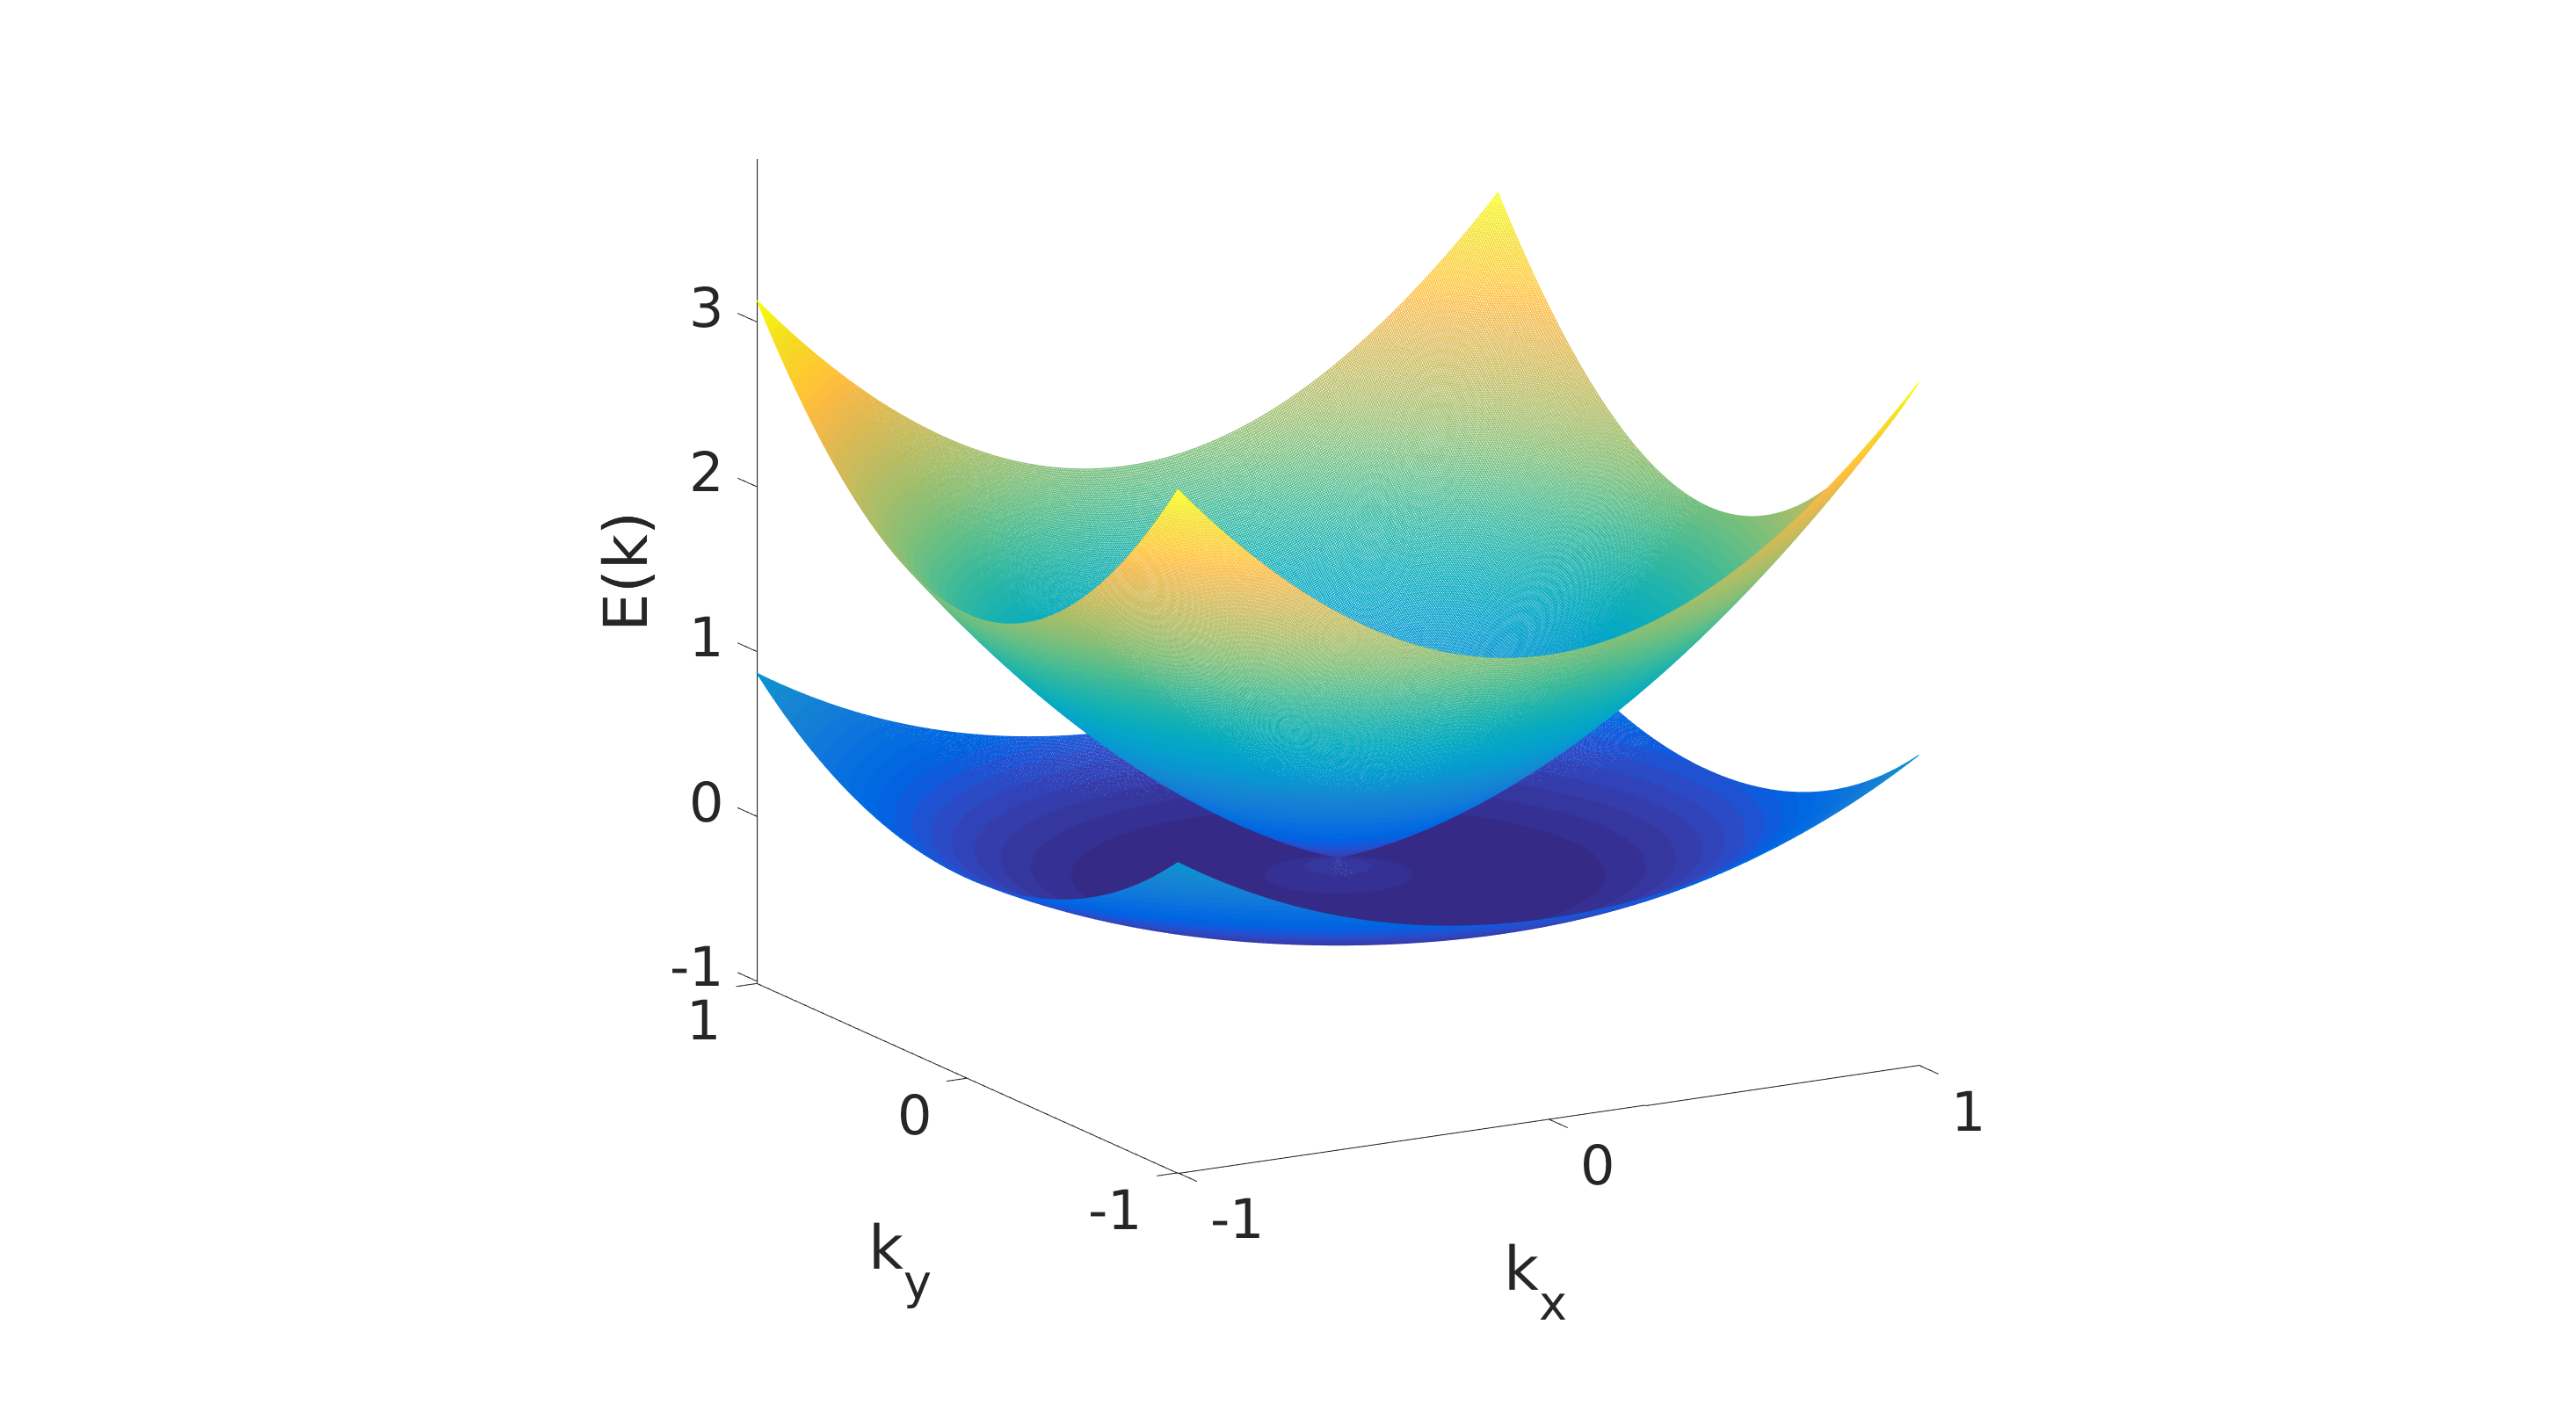
\includegraphics[width=12cm]{bands.eps}
	\caption{Band splitting by spin-orbit coupling}\label{bands}
\end{figure}

Let $\mathbf{k}=(k,\theta)$.
\begin{equation*}
H=\left(\begin{array}{cc}\frac{\hbar^2k^2}{2m}&i\alpha ke^{-i\theta}\\-i\alpha ke^{i\theta}&\frac{\hbar^2k^2}{2m}\end{array}\right)
\end{equation*}

The eigenvector for band $E_-(\mathbf{k})$ is
\begin{equation*}
|\Psi^-_{\mathbf{k}}\rangle=\frac{1}{\sqrt{2}}(1,ie^{i\theta})^T=\frac{1}{\sqrt{2}}|\mathbf{k}\rangle(|\uparrow\rangle+ie^{i\theta}|\downarrow\rangle)
\end{equation*}

The eigenvector for band $E_+(\mathbf{k})$ is
\begin{equation*}
|\Psi^+_{\mathbf{k}}\rangle=\frac{1}{\sqrt{2}}(1,-ie^{i\theta})^T=\frac{1}{\sqrt{2}}|\mathbf{k}\rangle(|\uparrow\rangle-ie^{i\theta}|\downarrow\rangle)
\end{equation*}

\subsection{Part (c)}
Since $E_{\pm}(\mathbf{k})$ depends only on $|\mathbf{k}|$, the Fermi surfaces are two concentric circles. $E_+$ corresponds to the smaller radius and $E_-$ corresponds to the larger radius. This is shown in Fig.\ref{Fermi}.
\begin{figure}[!htbp]
	\centering
	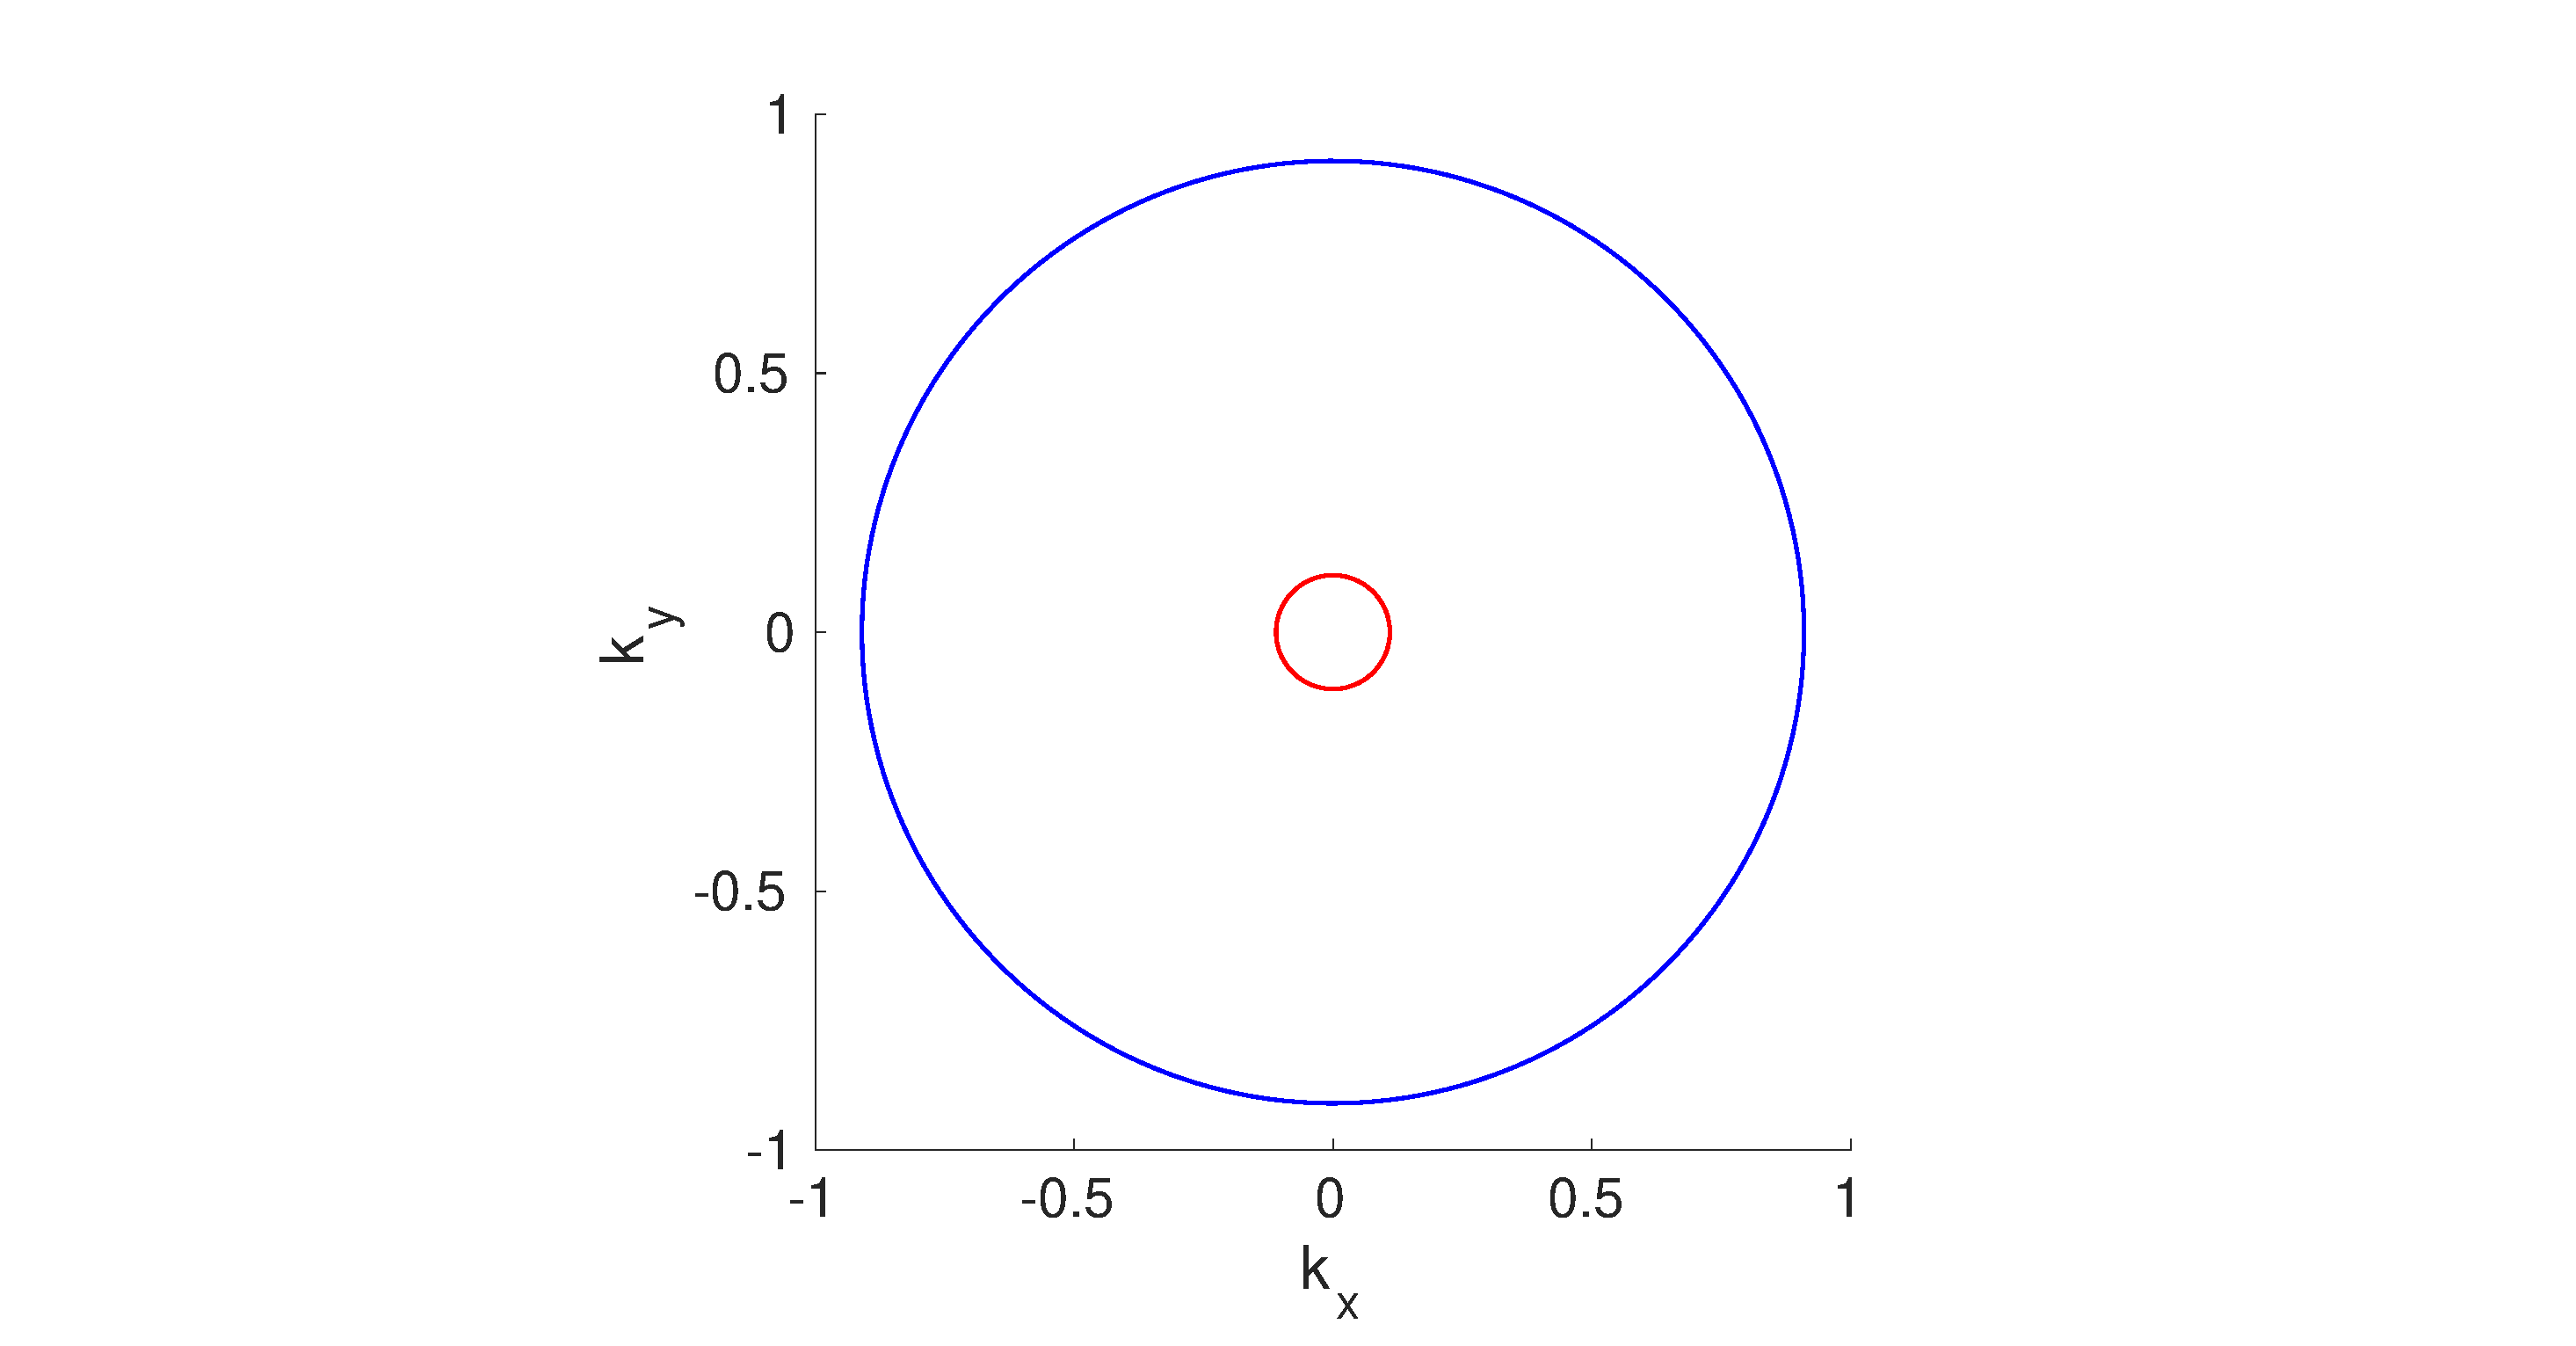
\includegraphics[width=12cm]{Fermi.eps}
	\caption{The Fermi surfaces}\label{Fermi}
\end{figure}

\begin{align*}
&\langle\Psi_{\mathbf{k}}^-|\sigma_x|\Psi_{\mathbf{k}}^-\rangle=\frac{1}{2}(1,-ie^{-i\theta})\left(\begin{array}{cc}0&1\\1&0\end{array}\right)\left(\begin{array}{c}1\\ie^{i\theta}\end{array}\right)=-\sin\theta\\
&\langle\Psi_{\mathbf{k}}^-|\sigma_y|\Psi_{\mathbf{k}}^-\rangle=\frac{1}{2}(1,-ie^{-i\theta})\left(\begin{array}{cc}0&-i\\i&0\end{array}\right)\left(\begin{array}{c}1\\ie^{i\theta}\end{array}\right)=\cos\theta\\
&\langle\Psi_{\mathbf{k}}^-|\sigma_z|\Psi_{\mathbf{k}}^-\rangle=\frac{1}{2}(1,-ie^{-i\theta})\left(\begin{array}{cc}1&0\\0&-1\end{array}\right)\left(\begin{array}{c}1\\ie^{i\theta}\end{array}\right)=0\\
&\langle\Psi_{\mathbf{k}}^+|\sigma_x|\Psi_{\mathbf{k}}^+\rangle=\frac{1}{2}(1,ie^{-i\theta})\left(\begin{array}{cc}0&1\\1&0\end{array}\right)\left(\begin{array}{c}1\\-ie^{i\theta}\end{array}\right)=\sin\theta\\
&\langle\Psi_{\mathbf{k}}^+|\sigma_y|\Psi_{\mathbf{k}}^+\rangle=\frac{1}{2}(1,ie^{-i\theta})\left(\begin{array}{cc}0&-i\\i&0\end{array}\right)\left(\begin{array}{c}1\\-ie^{i\theta}\end{array}\right)=-\cos\theta\\
&\langle\Psi_{\mathbf{k}}^+|\sigma_z|\Psi_{\mathbf{k}}^+\rangle=\frac{1}{2}(1,ie^{-i\theta})\left(\begin{array}{cc}1&0\\0&-1\end{array}\right)\left(\begin{array}{c}1\\-ie^{i\theta}\end{array}\right)=0
\end{align*}

Therefore,
\begin{align*}
\langle\mathbf{S}(\mathbf{k})\rangle|_{|\mathbf{k}|=k_F^-}&=-\frac{1}{2}\hat{\mathbf{k}}\times\hat{\mathbf{z}}\\
\langle\mathbf{S}(\mathbf{k})\rangle|_{|\mathbf{k}|=k_F^+}&=\frac{1}{2}\hat{\mathbf{k}}\times\hat{\mathbf{z}}
\end{align*}

On the inner circle ($E_+$), spin direction rotates clockwise. On the outer circle ($E_-$), spin direction rotates counterclockwise. This is shown in Fig.\ref{Fermi}.

\end{document}
